\documentclass[11pt]{beamer}
\usetheme{Warsaw}
\usepackage[utf8]{inputenc}
\usepackage[spanish]{babel}
\usepackage{amsmath}
\usepackage{amsfonts}
\usepackage{amssymb}
\usepackage{graphicx}
\author{N.Pérez-Medina}
\title{Capítulo 3 - \textbf{Interpolación y Extrapolación}}
\setbeamercovered{transparent} 
\setbeamertemplate{navigation symbols}{} 
\logo{
\includegraphics[scale=0.04]{logo_fing_uach_bn.png} } 
\institute{\textbf{FING - UACH}
	\\
	\begin{small}
	\textit{Resumen del libro 'Recetas Numéricas en C' de H. Press}\\
	\end{small}
	
	\bigskip
	
	\begin{small}
	\textbf{Catedrático:} Dr. José Luis Herrera Aguilar
	\end{small}		
	} 
\date{\today} 


% Para tener un morado coqueto
\definecolor{lightPurple}{RGB}{186, 146, 209} % Morado claro
\definecolor{darkPurple}{RGB}{98, 54, 150}    % Morado oscuro
\setbeamercolor{structure}{fg=darkPurple} % Color principal para estructuras
\setbeamercolor{frametitle}{bg=darkPurple, fg=white} % Título del marco
\setbeamercolor{block title}{bg=darkPurple, fg=white} % Título de bloques
\setbeamercolor{block body}{bg=lightPurple!30, fg=black} % Cuerpo de bloques

\begin{document}

\begin{frame}
\maketitle
\end{frame}

\begin{frame}
\tableofcontents
\end{frame}
\section{Contextualización}
\begin{frame}{Situación actual de Resultados de Investigación}
\begin{block}{\textbf{En general}}
Resultados \textit{inconsistentes}
\end{block}

\end{frame}
\section{Introducción}
\subsection{Idea central}
\begin{frame}{Idea general del capítulo}
Dado un conjunto de puntos conocidos 
$$ X := x_1,x_2,\dots,x_N $$ 
que suponemos ser evaluaciones de una $f(x)$ descionocida
\begin{block}{Cuando no tenemos una expresión analítica para $f(x)$}
\textbf{¿Qué queremos hacer?} Estimar $f(x)$ para un $x$ arbitrario.\\
 
\medskip

\textbf{¿Cómo?} Trazando, en algún sentido, una \textit{curva suave} a través de (y quizá más allá) de $X$
\end{block}
\end{frame}

\begin{frame}{Idea gráfica}
\centering
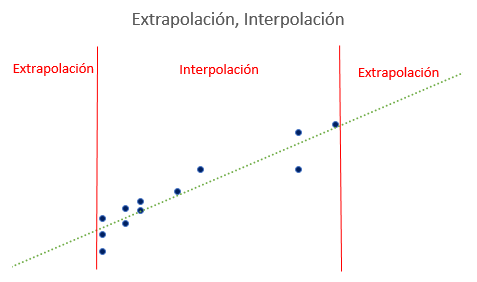
\includegraphics[scale=0.8]{extrapolacion-interpolacion.png} 
\end{frame}

\begin{frame}{Sobre las interpolaciones y extrapolaciones}
\begin{block}{Algunas opciones}
\begin{itemize}
\item Funciones trigonométircas
\item Funciones racionales
\item Polinomios
\end{itemize}
\end{block}

\begin{block}{Los teoremas al respecto}
Inútiles en nuestro contexto
\end{block}
\end{frame}
\subsection{Especificaciones}
\begin{frame}{Interpolación vs. Aproximación de funciones}

\begin{block}{En la \textbf{\textit{Interpolación}}}
Se te dan los valores de $f(x)$ en puntos que \textit{no has elejido tú mismo}
\end{block}

\begin{block}{En la \textbf{\textit{Aproximación de funciones}}}
Puedes calcular $f$ en cualquier conjunto de puntos deseado para el propósito de construir tu aproximación
\end{block}

\end{frame}

\begin{frame}{Funciones ''Patológicas''}

\begin{block}{Ejemplo}
$$
f(x) = 3x^2 + \frac{1}{\pi^4} \ln \left[ (\pi - x)^2 \right] + 1
$$
Es ''bien comportada'' en todo lugar excepto en $x=\pi$. 
\end{block}

\end{frame}

\begin{frame}{$f(x) = 3x^2 + \frac{1}{\pi^4} \ln \left[ (\pi - x)^2 \right] + 1$, (1/2)}
\centering
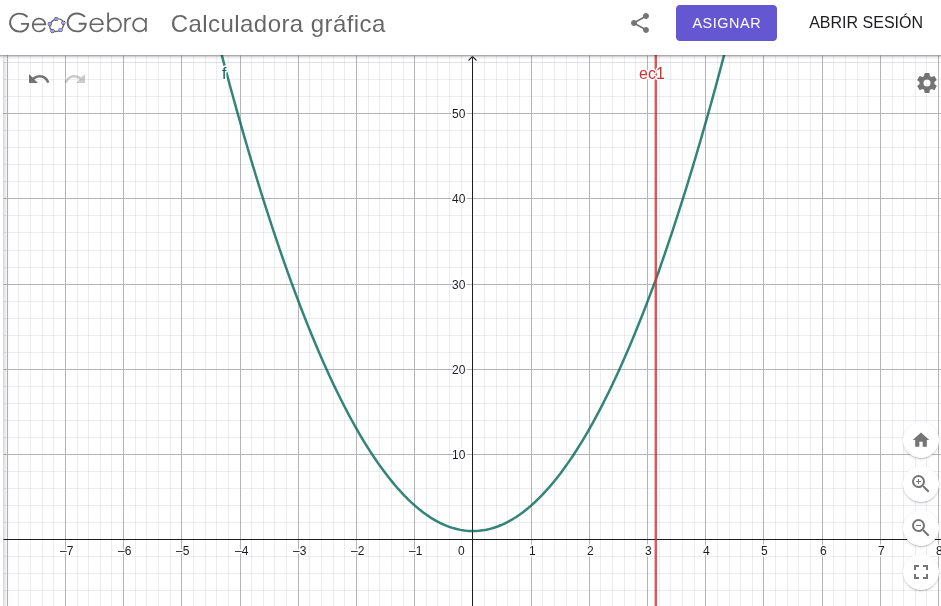
\includegraphics[scale=0.3]{f-pato.png} 
\end{frame}

\begin{frame}{$f(x) = 3x^2 + \frac{1}{\pi^4} \ln \left[ (\pi - x)^2 \right] + 1$, (2/2)}
\centering
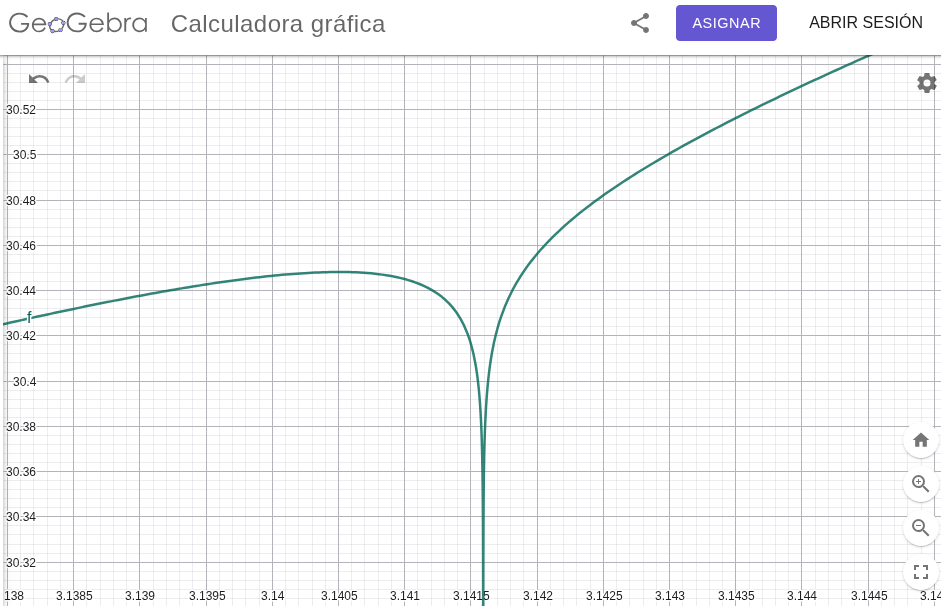
\includegraphics[scale=0.3]{zoom.png}  
\end{frame}

\begin{frame}{Importancia de las ''Patologías''}
\begin{block}{\textbf{Pueden esconderse en cualquier parte}}
Toda rutina de \textit{interpolación} o \textit{extrapolación} debe proporcionar una \textbf{estimación de su porpio error.}
\end{block}
\end{frame}
\subsection{Proceso ideal y real}
\begin{frame}{Concepto del \textit{proceso} de interpolación}
\begin{block}{\textbf{Etapa 1} - Ajustar una \textit{función de interpolación} a los datos proporcionados}
\begin{enumerate}
\item \textbf{Paso 1}
\item $\dots$
\item \textbf{Paso N}
\end{enumerate}
\end{block}
\begin{block}{\textbf{Etapa 2} - Evaluar dicha \textit{función} en el punto objetivo $x$}
\begin{enumerate}
\item \textbf{Paso 1}
\item $\dots$
\item \textbf{Paso M}
\end{enumerate}
\end{block}

\end{frame}

\begin{frame}{Concepto del \textit{proceso} de interpolación}
\centering
\begin{Huge}
\textbf{¡Pues no es cierto!}\footnote{Computacionalmente hablando}
\end{Huge}
\end{frame}

\begin{frame}{Concepto del \textit{proceso} de interpolación}
\centering
\begin{Huge}
\textbf{¡Pues no es cierto!}\footnote{Computacionalmente hablando}
\end{Huge}

\begin{block}{¿Porqué?}
En términos generales es:
\begin{enumerate}
\item Menos eficiente
\item Suceptible a errores de redondeo
\end{enumerate}
\end{block}
\begin{block}{\textbf{Recomendación general}}
Los \textit{coeficientes} de un polinomio interpolador son de interés, pero \textbf{su uso al evaluar la función interpolada se desaconseja}
\end{block}
\end{frame}



\begin{frame}{Concepto realista del \textit{proceso} de interpolación}
\begin{block}{En la mayoria de los esquemas}
\begin{itemize}
\item Comenzamos con un valor cercano $f(x_i)$
\item Agregamos una serie de correcciones al mismo tiempo que incorporamos otros valores $f(x_i)$
\end{itemize}
La última correción será la más pequeña, y puede usarse como cota formal del error.
\end{block}

\end{frame}

\subsection{Interpolación local y \textit{spline}}

\begin{frame}{Idea gráfica 1}
\centering
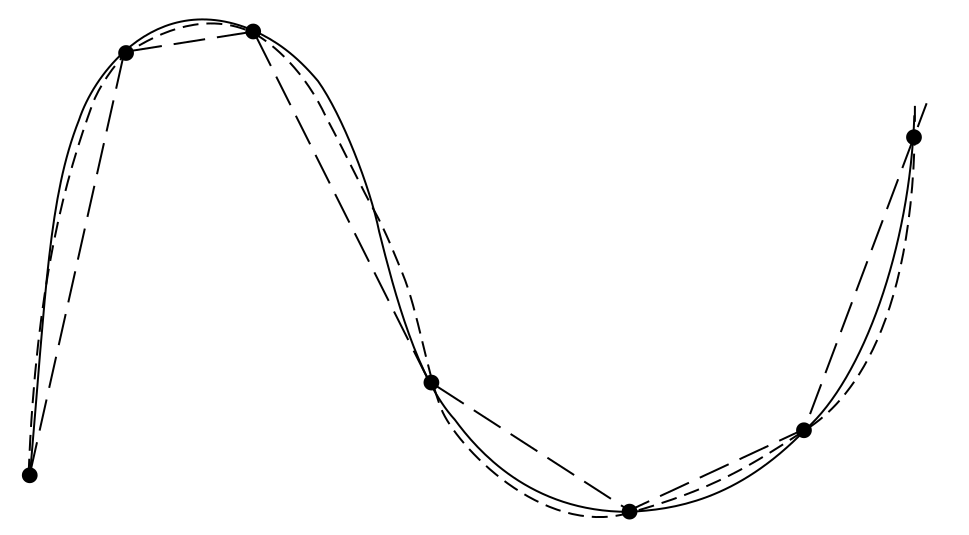
\includegraphics[scale=0.3]{c1.png} 
\end{frame}

\begin{frame}{\textit{spline}}
\begin{block}{En general}
Un \textit{spline} es un polinomio entre cada par de puntos tabulados, pero cuyos coeficientes se determinan de forma ''ligeramente'' no local.
\end{block}

\begin{block}{Ventajas}
Esa ''no localidad'' está diseñada para garantizar la \textit{suavidad} en la función interpolada.
\end{block}
\end{frame}

\begin{frame}{Orden de interpolación}
\begin{block}{Definición}
El número de puntos (menos uno) utilizados en un esquema de interpolaciṕon se llama el \textit{orden} de interpolación
\end{block}

\begin{block}{Generalidades}
\begin{itemize}
\item Aumentar el orden \textbf{no} necesariamente mejora la precisión
\item Se recomiendan grados de 3, 4 o hasta 6
\item Para más puntos hace falta monitoreo constante y riguroso del error estimado 
\end{itemize}
\end{block}
\end{frame}

\begin{frame}{Idea gráfica 2}
\centering
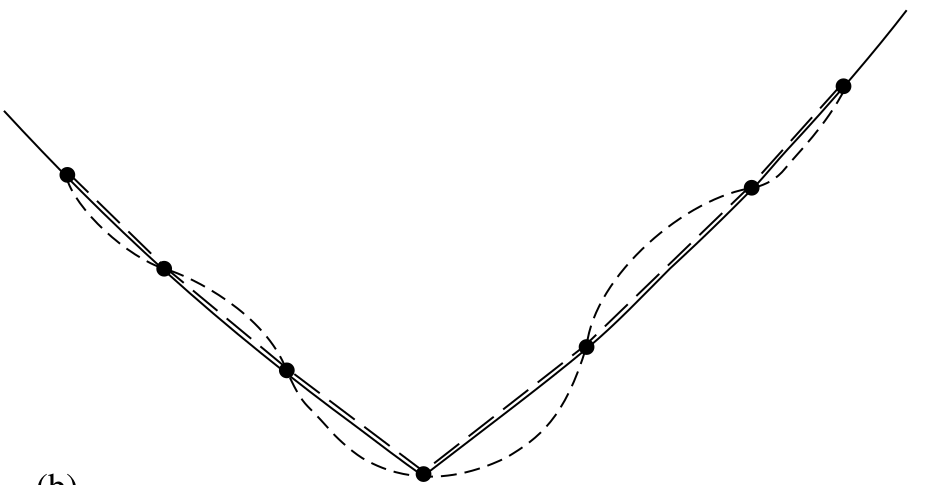
\includegraphics[scale=0.3]{c2.png} 
\end{frame}

\section*{Gracias}
\begin{frame}{Por su atención}
\centering
\begin{Huge}
Gracias \\
\end{Huge}

\includegraphics[scale=0.1]{gracias.jpg} 
\end{frame}

\end{document}

